%% Manuscript for Advances in Space Research (Elsevier/COSPAR), section EM (Earth's magnetosphere / space weather).
%% Template: Elsevier CAS double-column (cas-dc; double-column is allowed for LaTeX submissions), author-year
%% references (cas-model2-names). For a single-column version change cas-dc to cas-sc (cas-sc.cls is included).
%% Compile with pdfLaTeX + BibTeX (Overleaf: Menu -> Compiler: pdfLaTeX).
%% tables/ and figures/ are generated by pipeline/journal_tables.py and journal_figures.py of
%% https://github.com/bnsama29-cloud/STORM-PhysNet-L2 . \pend marks results of the last Kaggle campaign (campaign 2).
\documentclass[a4paper,fleqn]{cas-dc}

\usepackage[authoryear,longnamesfirst]{natbib}
\usepackage{amsmath,amssymb}
\usepackage{booktabs}
\usepackage{adjustbox}
\usepackage{xcolor}
\emergencystretch=2em

\newcommand{\pend}{\textcolor{red}{[pending]}}
\newcommand{\PE}{\mathrm{PE}}

\begin{document}
\let\WriteBookmarks\relax
\def\floatpagepagefraction{1}
\def\textpagefraction{.001}

\shorttitle{Physics-guided vs data-driven forecasts of GEO relativistic electrons}
\shortauthors{Samarth B N}

\title [mode = title]{Physics-guided versus data-driven forecasts of relativistic electrons at geostationary
orbit: skill, robustness and transfer across four satellites}

\author[1]{Samarth B N}
\cormark[1]
\ead{samarthbn.ec25@rvce.edu.in}
\credit{Conceptualization, Methodology, Software, Validation, Formal analysis, Investigation, Data curation,
Writing -- original draft, Writing -- review \& editing, Visualization}

\affiliation[1]{organization={Department of Electronics and Communication Engineering, RV College of Engineering},
            addressline={Mysore Road},
            city={Bengaluru},
            postcode={560059},
            state={Karnataka},
            country={India}}

\cortext[1]{Corresponding author}

\begin{abstract}
Electrons above 2\,MeV at geostationary orbit charge spacecraft dielectrics, and forecasts are needed also at
longitudes that no GOES satellite monitors. We compare STORM-PhysNet, a forecast network with a learned
solar-wind delay, a gate driven by the southward interplanetary magnetic field, outputs relative to
persistence and a physics-informed loss, with 18 other model families. All are trained on hourly GOES-15 data
(2010--2020) to forecast 1, 6, 12 and 24\,h ahead, with ten random seeds on each of three disjoint test periods
and a protocol that prevents information leakage; differences are tested with paired \(t\)-tests. Predicting
the change from persistence gives the 1\,h skill, and solar-wind inputs give the 6--24\,h skill. The delay,
the gate, the physics loss, two alternative gates, a spectral head and magnetopause features change no score
significantly. The encoder matters more: with a long short-term memory (LSTM) encoder, STORM-PhysNet has the
highest 1\,h skill of all models (prediction efficiency 0.975), matches the best at 6\,h (0.852), is the most
robust to input noise and missing solar-wind data, and transfers best without retraining to GOES-16 and
GOES-18, at a cost of 0.016 at 24\,h. Models that forecast the flux level directly lose their skill on GOES-16,
whose flux reads a factor of two lower than GOES-15, whereas models that forecast the change keep part of it.
With local data, fine-tuning brings all models to similar skill on GOES-16, GOES-18 and India's GSAT-19.
\end{abstract}

\begin{highlights}
\item Twenty forecast models compared on three test periods, ten seeds and paired tests.
\item Persistence residual explains 1\,h skill; solar-wind drivers explain 6--24\,h skill.
\item Physics-inspired delay, gates and losses do not change accuracy significantly.
\item An LSTM encoder makes the physics-guided model the most robust and transferable.
\item Forecasting changes, not levels, survives a factor-of-two satellite offset.
\end{highlights}

\begin{keywords}
Radiation belts \sep Relativistic electrons \sep Geostationary orbit \sep Space weather \sep
Machine learning \sep Transfer learning
\end{keywords}

\maketitle

%% =====================================================================================================
\section{Introduction}
\label{sec:intro}
%% =====================================================================================================
Electrons with energies above 2\,MeV in the outer radiation belt penetrate spacecraft shielding and
accumulate in insulating materials. When the flux stays high for a day or more, the stored charge can
discharge inside electronics, and anomalies of geostationary (GEO) satellites cluster after such
enhancements \citep{baker2018}. The flux can rise by orders of magnitude within a day after a geomagnetic
disturbance, through wave--particle acceleration in the inner magnetosphere \citep{horne2005}. Operators
therefore need forecasts hours ahead. NOAA issues an alert when the \(>2\)\,MeV flux measured by its GOES
satellites exceeds 1000\,pfu (particles cm\(^{-2}\)\,s\(^{-1}\)\,sr\(^{-1}\)), but GOES satellites sit over the
Americas, and many GEO satellites, including India's INSAT and GSAT series, operate at longitudes where the flux
differs.

Forecasting has progressed from linear prediction filters driven by solar-wind speed \citep{baker1990} and
empirical models \citep{perry2010} to neural networks \citep{wei2018,son2022} and Transformers
\citep{tan2024,sun2024,sun2025}. Two problems limit how far these results can be trusted and used. First,
evaluation choices such as interpolating across data gaps, smoothing with filters that look ahead,
interleaving training and test months and testing on a single year can inflate skill
\citep{camporeale2019,kapoor2023}. Few studies report the variability between training runs or test whether
differences are significant, and simple models often rival Transformers \citep{zeng2023,tan2024}. Second,
models are almost always trained and tested on a single satellite \citep{zhao2025}, so it is unclear how they
behave on another instrument or at another longitude.

This paper evaluates a physics-guided forecast network, STORM-PhysNet, under a strict protocol and against a
wide set of controls. A shorter version was accepted at a conference (AGERS 2026) and withdrawn before
publication. The present study adds a 24\,h lead time; ten further model families, so that every
physics-inspired component is compared with a model that lacks only that component; probabilistic,
storm-time and alert-level scores; robustness tests that mimic operational data failures; and transfer to
three other satellites: GOES-16 at a different longitude, GOES-18 at the same longitude as GOES-15, and the
GRASP spectrometer on India's GSAT-19 at 48\(^\circ\)E. The contribution is less a new architecture than a
test of which components help, at which lead time, and on which satellite.

%% =====================================================================================================
\section{Related work}
\label{sec:related}
%% =====================================================================================================
Linear prediction filters relate GEO electron flux to the solar-wind speed of the preceding days
\citep{baker1990} and underlie NOAA's operational Relativistic Electron Forecast Model. Comparing several such
models, \citet{perry2010} found no clear winner and a strong dependence of skill on the solar cycle.
\citet{wei2018} forecast the daily \(>2\)\,MeV flux one day ahead with a long short-term memory (LSTM) network
\citep{hochreiter1997}. \citet{son2022} forecast hourly flux 1--72\,h ahead with a multilayer perceptron, using
a split that interleaves months of the same year. \citet{forsyth2020} framed GOES-15 forecasting as the
exceedance of flux thresholds and found persistence hard to beat at the lower threshold. \citet{tan2024}
found a Transformer only slightly, and not significantly, better than an attention-based LSTM, and
\citet{sun2024,sun2025} compared LSTM and Transformer models at lead times of 1--24\,h and improved daily
fluence prediction with pre-training. None of these studies reports significance tests over repeated training
runs. The Temporal Fusion Transformer \citep{lim2021} already combines gating with forecasts at several lead
times; our gate differs mainly in being conditioned on the interplanetary magnetic field.

On evaluation, skill should be reported against persistence as well as climatology
\citep{camporeale2019,morley2018}; information leaking from the test period into training is a common cause
of results that do not reproduce \citep{kapoor2023}; and ordinary cross-validation suits time series only when
the errors are uncorrelated \citep{bergmeir2018}. For probabilistic forecasts, proper scoring rules such as the
continuous ranked probability score (CRPS) assess calibration and sharpness together \citep{gneiting2007}.
Across satellites, \citet{zhao2025} merged cross-calibrated FY-4A and GOES-15 records for training, and
\citet{rodriguez2025} assessed the consistency of GOES-8 to GOES-15 electron fluxes. We know of no study that
compares zero-shot use, fine-tuning and training from scratch on new GEO sensors.

%% =====================================================================================================
\section{Data}
\label{sec:data}
%% =====================================================================================================
\subsection{GOES-15 electron flux}
The training data and the main test data are the \(>2\)\,MeV integral electron flux of the Energetic Proton,
Electron and Alpha Detector on GOES-15 \citep{goes15_epead}, from 2010 to March 2020, at 135\(^\circ\)W for
most of the period. We average the measurements to hourly means (87\,168 hours) and take the base-10
logarithm, so that the models work with orders of magnitude rather than raw values. The standard deviation of
the measurements within each hour is kept as an extra input, because it indicates how fast the flux is
changing.

\subsection{Solar-wind and geomagnetic drivers}
The hourly OMNI data set \citep{king2005,omni2020} provides the solar-wind speed, the north--south
component \(B_z\) and magnitude of the interplanetary magnetic field (IMF), the proton density and the
dynamic pressure, already propagated to the nose of Earth's bow shock, together with the Kp and Dst
geomagnetic indices. From these we derive seven further channels: the number of consecutive hours with
southward \(B_z\), the time since the start of the current storm, running means of the speed over 1, 6 and
24\,h and of \(B_z\) over 1 and 6\,h, and the product of speed and \(B_z\), a simple measure of the energy
the solar wind couples into the magnetosphere. With the flux, its within-hour spread and a mask that marks
observed hours, each forecast sees 18 channels over the preceding 72\,h.

\subsection{GOES-16 and GOES-18}
For the transfer experiments we use the level-2 five-minute \(>2\)\,MeV integral electron flux of the
Magnetospheric Particle Sensor (MPS-HI) of the Space Environment In Situ Suite \citep{kress2020} on GOES-16 and
GOES-18 \citep{ncei_goesr}. MPS-HI has five telescopes arranged in a north--south fan; we use telescope 4, the
middle of the fan, which stays nearest the equatorial plane also when the spacecraft is flipped. Hours with at
least six valid five-minute values are kept. GOES-16 (GOES-East, 75.2\(^\circ\)W) gives 50\,598 hours from
January 2017 to April 2025, and GOES-18 (GOES-West, 137\(^\circ\)W) gives 34\,578 hours from April 2022 to
November 2026. Over the 19\,138 hours observed by both GOES-15 and GOES-16 (January 2017 to March 2020), the
GOES-16 flux is lower by a median of 0.30 in \(\log_{10}\) (a factor of two), while daily means correlate at
0.98 (Fig.~\ref{fig:g15g16}). We deliberately do not cross-calibrate the two records: the transfer experiments
test how forecasts cope with exactly such an offset.

\subsection{GSAT-19 GRASP}
The Geostationary Radiation Spectrometer (GRASP) on GSAT-19 at 48\(^\circ\)E provides \(>2\)\,MeV flux from
July 2017 to August 2018 (10\,249 hours, of which 10\,158 are observed), distributed by the Indian Space Science
Data Centre \citep{grasp_issdc}. As in the conference study, every driver channel of the GRASP inputs is held at
its GOES-15 training mean, so this experiment tests the transfer of the flux-history part of each model under a
change of instrument and longitude.

\begin{figure*}[!t]
\centering
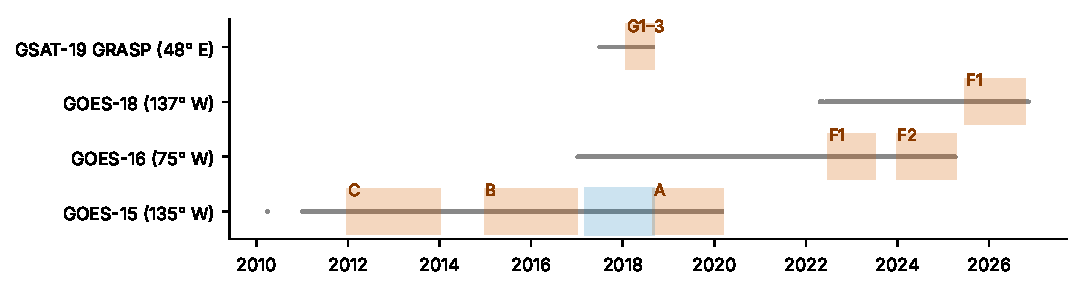
\includegraphics[width=\textwidth]{figures/fig_data.pdf}
\caption{Data and evaluation design. Grey: hours with flux data on each satellite. Orange: test periods
(GOES-15 blocks A--C, GOES-16 folds F1--F2, GOES-18 fold F1 and GRASP folds G1--G3). Blue: the shared GOES-15
validation period.}
\label{fig:data}
\end{figure*}

\begin{figure}[!t]
\centering
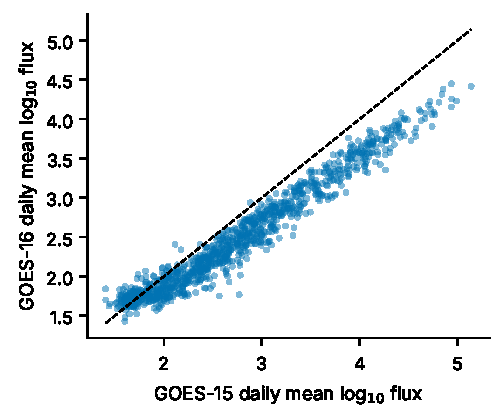
\includegraphics[width=\columnwidth]{figures/fig_g15_g16.pdf}
\caption{Daily mean \(\log_{10}\) flux of GOES-16 against GOES-15 over their 2017--2020 overlap. Dashed line:
equality. GOES-16 reads 0.30 lower in \(\log_{10}\) (median of the hourly differences).}
\label{fig:g15g16}
\end{figure}

%% =====================================================================================================
\section{Evaluation protocol}
\label{sec:protocol}
%% =====================================================================================================
\subsection{Preventing information leakage}
Four choices keep information from the future or from the test period out of the inputs.
(1) Missing GOES hours (27--32\% of training hours) are filled forward from earlier hours only, never
interpolated; the mask channel tells the model which hours are real, and a forecast window is scored only if
its last input hour and all four target hours are real observations. (2) No smoothing or despiking filter
that uses later values is applied. (3) OMNI repeats each three-hourly Kp value on all three hours, which would
reveal up to two hours of the future; each hour therefore sees only the last completed Kp interval.
(4) A window is used only if all 96 of its hours (72 input hours plus the 24\,h lead time) belong to the same
part of the split, which leaves a 96\,h gap at every boundary. The input scaling is computed from training
hours only.

\subsection{Test blocks}
Three GOES-15 test blocks share one validation period (March 2017 to September 2018). For each block, every
model is trained again on all remaining hours (Fig.~\ref{fig:data}). Block A (September 2018 to March 2020;
7\,143 test windows) comes after its training and validation data, so it is a strictly chronological test.
Blocks B (2015--2016; 13\,431 windows) and C (2012--2013; 12\,362 windows) contain the strong storms of 2015 and
2012--2013 and have training data on both sides; they are a form of blocked cross-validation
\citep{bergmeir2018}. Blocks B and C hold most of the storm-time targets (Dst \(\le-50\)\,nT): 290--617 per lead
time and block, against 13--32 in block A.

\subsection{Scores}
\label{sec:scores}
The main score is the prediction efficiency (PE), the fraction of the target variance that a forecast
explains, relative either to climatology or to persistence:
\begin{align}
\PE_{\mathrm{clim}} &= 1 - \mathrm{MSE}(\hat y, y)/\mathrm{Var}(y), \label{eq:peclim}\\
\PE_{\mathrm{pers}} &= 1 - \mathrm{MSE}(\hat y, y)/\mathrm{MSE}(y_t, y), \label{eq:pepers}
\end{align}
where \(y\) is the observed \(\log_{10}\) flux at the target hour, \(\hat y\) the forecast, \(y_t\) the last
observed value and MSE the mean squared error. \(\PE_{\mathrm{clim}}=1\) is a perfect forecast and 0 is no
better than always forecasting the mean; \(\PE_{\mathrm{pers}}>0\) means the forecast beats persistence. PE
without a subscript means \(\PE_{\mathrm{clim}}\). We also report the root-mean-square error (RMSE) of
\(\log_{10}\) flux at storm time (Dst \(\le-50\)\,nT at the target hour), and the Heidke skill score (HSS)
\citep{jolliffe2011} for the event that the flux exceeds the 1000\,pfu alert level (1 for perfect event
forecasts, 0 for no skill beyond chance). For models that also predict an uncertainty \(\hat\sigma\), we report
how often the observation falls inside \(\hat y\pm\hat\sigma\) and \(\hat y\pm1.96\hat\sigma\) (68\% and 95\%
if the uncertainty is right) and the CRPS of the Gaussian forecast \(\mathcal N(\hat y,\hat\sigma^2)\)
\citep{gneiting2007}, which is in units of \(\log_{10}\) flux and smaller for better forecasts.

\subsection{Statistics}
Every model is trained with ten random seeds (42--51) in every block, so that differences between models can
be compared with the spread caused by random initialisation and data shuffling alone. Because the same seeds
recur in every block, the 30 seed--block results are not independent. The main test therefore averages each
seed's difference between two models over the three blocks and applies a paired \(t\)-test to the ten seed
means. When a table holds many comparisons, the \(p\)-values are adjusted with the Holm method, which controls
the chance of any false positive across the whole table. Figures show 95\% confidence intervals of the mean
difference over seeds.

\subsection{Robustness tests}
The test inputs are degraded in ways that mimic operational failures: Gaussian noise with standard deviation
\(\sigma=0.5\), 1 and 2 (in units of each standardised channel) added to every channel except the observed-hour
mask; driver channels frozen at their last value for the final 6 or 24 input hours, as during an outage of the
upstream solar-wind monitor; driver channels set to their training mean for the whole input, as if no driver
data existed; and Kp and Dst arriving three hours late.

\subsection{Transfer to other satellites}
The block-A GOES-15 models, trained on data up to March 2017 and validated up to September 2018, are applied to
the other satellites in four ways: \emph{zero-shot}, without any retraining; \emph{heads}, retraining only the
output layers with the encoder frozen; \emph{full}, fine-tuning all weights; and \emph{scratch}, training the
same architecture on the target satellite alone. All folds are chronological, and every target window lies
after the GOES-15 validation period. For GOES-16, fold F1 trains on September 2018 to December 2021, validates
on January--June 2022 and tests on July 2022 to June 2023; fold F2 trains to June 2023, validates on
July--December 2023 and tests on January 2024 to April 2025, which includes the storm of May 2024
\citep{pierrard2024}. For GOES-18, the model trains on April 2022 to December 2024, validates on
January--June 2025 and tests on July 2025 to October 2026. GRASP uses the three folds of the conference study,
with tests in February--March, April--May and June--August 2018. Fine-tuning minimises the mean squared error
weighted by lead time, with the Adam optimiser (learning rate \(10^{-4}\), or \(3\times10^{-4}\) from scratch)
and early stopping on the fold's validation data.

%% =====================================================================================================
\section{Models}
\label{sec:models}
%% =====================================================================================================
\begin{figure*}[!t]
\centering
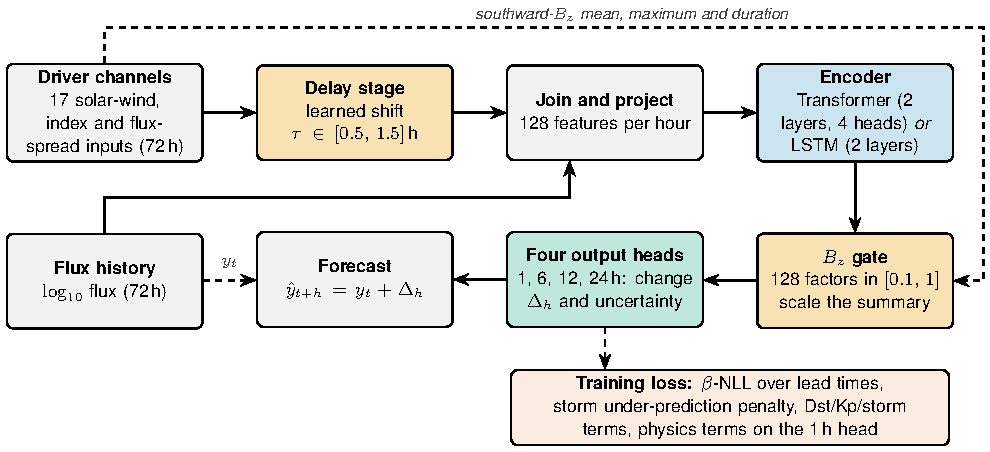
\includegraphics[width=\textwidth]{figures/fig_architecture.pdf}
\caption{STORM-PhysNet. Orange: the physics-inspired components tested in this study (delay stage and \(B_z\)
gate); blue: the encoder, a Transformer in the original model and an LSTM in the best variant; green: one output
head per lead time, each predicting a change from persistence and its uncertainty. The diagram was drawn in TikZ
with code written with the assistance of Claude Opus 5.5 (Anthropic) and checked by the author against the model code.}
\label{fig:arch}
\end{figure*}

\subsection{STORM-PhysNet}
STORM-PhysNet (Fig.~\ref{fig:arch}; 360\,227 parameters with four lead times) processes a 72\,h input window in
four steps.

\emph{Delay stage.} The OMNI data are propagated to the bow shock with an assumed solar-wind speed, so the
timing of each solar-wind feature may still be off by about an hour. A small network looks at the window and
outputs a delay \(\tau\) between 0.5 and 1.5\,h. Each hour of the 17 auxiliary channels is then replaced by a
linear interpolation between the values \(\lfloor\tau\rfloor\) and \(\lfloor\tau\rfloor+1\) hours earlier,
all inside the window, so no future value is used. At \(\tau=1.5\)\,h this is simply the average of hours
\(t-1\) and \(t\).

\emph{Encoder.} The delayed channels and the flux history are joined, projected to 128 features per hour and
passed through an encoder that summarises the whole window. In the original model the encoder is a
Transformer \citep{vaswani2017} with two layers, four attention heads and a feed-forward width of 256: every
hour can attend directly to every other hour. In the LSTM variant it is a two-layer LSTM \citep{hochreiter1997}
of the same width, which reads the window hour by hour and carries a memory forward in time.

\emph{\(B_z\) gate.} A southward IMF \(B_z\) lets solar-wind energy enter the magnetosphere and usually
precedes electron enhancements. The gate is a small network of three numbers: the mean and the maximum of the
southward part of \(B_z\) in the window and the current southward-\(B_z\) duration. It outputs 128 factors
between 0.1 and 1 that scale the encoder's summary, so that the model can emphasise or suppress features
according to the driving.

\emph{Residual heads.} One head per lead time \(h\) predicts a change \(\Delta_h\) and a log-variance. The
forecast is \(\hat y_{t+h}=y_t+\Delta_h\): the network learns how much the flux will change from its last
observed value, rather than the value itself.

\emph{Loss.} The training loss is a \(\beta\)-weighted Gaussian negative log-likelihood \citep{seitzer2022},
which fits both the forecast and its uncertainty, averaged over the lead times with weights 1, 0.7, 0.5 and
0.4. It adds a 2.5-fold penalty when the forecast falls short during storms, auxiliary terms that predict Dst,
Kp and a storm class, and three physics-informed terms on the 1\,h head that switch on after a warm-up: a bound
on how fast the flux can respond to the energy input, a term that rewards a response to southward \(B_z\), and
a term that keeps the forecast change consistent with the Akasofu \(\epsilon\) coupling function. Training uses
the AdamW optimiser (learning rate \(3\times10^{-4}\) with cosine decay, batch size 64, at most 40 epochs,
early stopping on the validation error) and samples storm windows twelve times more often than quiet ones.

\subsection{Variants}
Each variant changes one component of STORM-PhysNet. \emph{No delay}: the delay stage is removed. \emph{Fixed
average}: the learned delay is replaced by the fixed average of hours \(t-1\) and \(t\). \emph{No gate}: the
gate is bypassed. \emph{No physics loss}: the three physics-informed terms are removed. \emph{Cathode--anode
gate}: the gate is replaced by an ``emission'' network of speed, southward \(B_z\) and field magnitude,
multiplied by a learned transmittance per feature. \emph{Cathode--anode + spectral}: the same gate plus a head
that predicts the parameters of a kappa energy spectrum, trained through an additional loss term.
\emph{Radiotrophic gate}: a gate that responds, with saturation, to an exponentially weighted ``dose'' of
driving. \emph{LSTM encoder}: the Transformer encoder is replaced by the two-layer LSTM. \emph{Magnetopause}:
features of the \citet{shue1998} magnetopause stand-off distance, computed in physical units from the latest
dynamic pressure and \(B_z\), are added to the encoder's summary. A second campaign removes the gate, the
delay or the physics loss from the LSTM variant, and trains an LSTM that has the persistence residual but none
of the other STORM-PhysNet components \pend.

\subsection{Controls}
All controls use the same data, sampler and training code. \emph{Matched Transformer} (1.19\,M parameters):
STORM-PhysNet's width, depth and heads with a feed-forward width of 2048, without delay, gate or residual.
\emph{Default Transformer}: a smaller configuration (64 features per hour, three layers). \emph{Transformer,
FFN 256}: feed-forward width 256, no residual. \emph{Residual Transformer} (268\,k parameters): feed-forward
width 256 with the persistence residual but no delay or gate; also trained with the fixed two-hour average on
its driver channels. \emph{Flux-only Transformer}: the matched Transformer with every driver channel set to
zero. \emph{Baselines}: an LSTM (two layers of 64 units), a multilayer perceptron (MLP) and a one-dimensional
convolutional network (CNN), all predicting the flux level directly. The 19 families make 570 training runs,
which took about 42 GPU-hours on NVIDIA T4 GPUs.

\subsection{Software and use of AI tools in the research}
All models, training, evaluation, statistics and figures are implemented in Python with PyTorch, NumPy, SciPy and
Matplotlib; Fig.~\ref{fig:arch} is drawn with TikZ. The author wrote and edited this code with the assistance of
the generative AI tool Claude (Anthropic; models Claude Opus 5.5 and Claude Sonnet 5.5), which was used to write
and revise the data pipeline, model, training, statistics and plotting code and to cross-check reported numbers
against the result files. All design choices were made by the author. The code is covered by automated tests
(56 tests, including tests that each model variant changes only its intended component and that the fixed
delay average uses no future values), every figure and table is generated directly from the saved predictions by the published
scripts, and all results can be reproduced from the repository given under Data and code availability.

%% =====================================================================================================
\section{Results}
\label{sec:results}
%% =====================================================================================================
\subsection{Skill on GOES-15}
\label{sec:skill}
Table~\ref{tab:main} and Fig.~\ref{fig:horizon} summarise the test skill. Every model except the CNN beats
persistence clearly at 6 and 12\,h. At 1\,h persistence is already strong (0.967), and only the models that
forecast the change from persistence improve on it: the STORM-PhysNet family and the residual Transformers reach
0.971--0.975 (\(\PE_{\mathrm{pers}}=0.13\)--0.25), whereas every model that forecasts the flux level directly
stays below persistence (at most 0.962). At 6 and 12\,h the Transformer controls that see the solar-wind drivers
lead (about 0.85 and 0.80, whatever their size or head), together with the LSTM variant of
STORM-PhysNet at 6\,h (0.852); the original STORM-PhysNet trails them by 0.034--0.053, which is significant at
12\,h after Holm adjustment (Table~\ref{tab:paired}). The MLP is close behind the Transformers (0.842 and 0.796)
and the LSTM baseline slightly further, while the CNN is far weaker at every lead time. At 24\,h the strong
models lie within 0.02 of each other (0.72--0.74), with the residual Transformer highest (0.741). The
chronological block A gives the same ranking (Table~\ref{tab:blockA}), and Fig.~\ref{fig:scatter} shows that
the 12\,h forecasts follow the observations over four orders of magnitude.

Persistence scores higher at 24\,h (0.546) than at 12\,h (0.249). The flux seen at a fixed position on GEO
follows a daily cycle in local time, so the value 24\,h earlier, taken at the same local time, is a better
guess than the value 12\,h earlier, taken on the opposite side of the orbit. A 24\,h forecast must therefore
beat a stronger reference than a 12\,h forecast, and the strong models do so by 0.17--0.20.

\begin{table*}[!t]
\centering
\caption{GOES-15 test skill, $\mathrm{PE}_\mathrm{clim}$: mean over ten seeds and the three test blocks.}
\label{tab:main}
\footnotesize
\setlength{\tabcolsep}{4pt}
\begin{adjustbox}{max width=\linewidth}
\begin{tabular}{lcccc}
\toprule
Model & 1\,h & 6\,h & 12\,h & 24\,h \\
\midrule
\multicolumn{5}{l}{\textit{Reference}} \\
Persistence & 0.967 & 0.572 & 0.249 & 0.546 \\
\multicolumn{5}{l}{\textit{Classical baselines}} \\
Ridge regression, residual & 0.976 & 0.848 & 0.794 & 0.745 \\
Gradient-boosted trees, residual & \pend{} & \pend{} & \pend{} & \pend{} \\
\multicolumn{5}{l}{\textit{Baselines}} \\
LSTM & 0.929 & 0.833 & 0.791 & 0.726 \\
LSTM, residual & 0.974 & 0.849 & 0.789 & 0.732 \\
\quad width 64 & \pend{} & \pend{} & \pend{} & \pend{} \\
\quad width 256 & \pend{} & \pend{} & \pend{} & \pend{} \\
MLP & 0.932 & 0.842 & 0.796 & 0.718 \\
CNN & 0.766 & 0.608 & 0.547 & 0.519 \\
\multicolumn{5}{l}{\textit{Transformer controls}} \\
Transformer (default size) & 0.958 & 0.850 & 0.802 & 0.733 \\
Transformer, matched & 0.961 & 0.848 & 0.797 & 0.737 \\
Transformer, FFN 256 & 0.960 & 0.849 & 0.799 & 0.737 \\
Residual Transformer & 0.972 & 0.850 & 0.798 & 0.741 \\
\quad + fixed average & 0.972 & 0.847 & 0.795 & 0.738 \\
Flux-only Transformer & 0.962 & 0.823 & 0.747 & 0.646 \\
\multicolumn{5}{l}{\textit{STORM-PhysNet and variants}} \\
STORM-PhysNet & 0.972 & 0.814 & 0.749 & 0.731 \\
\quad fixed average & 0.971 & 0.811 & 0.745 & 0.733 \\
\quad no delay & 0.971 & 0.814 & 0.748 & 0.736 \\
\quad no gate & 0.972 & 0.818 & 0.754 & 0.732 \\
\quad no physics loss & 0.973 & 0.824 & 0.759 & 0.730 \\
\quad physical-unit loss & \pend{} & \pend{} & \pend{} & \pend{} \\
\quad cathode--anode gate & 0.972 & 0.824 & 0.755 & 0.730 \\
\quad cathode--anode + spectral head & 0.971 & 0.816 & 0.753 & 0.735 \\
\quad radiotrophic gate & 0.971 & 0.807 & 0.746 & 0.733 \\
\quad LSTM encoder & 0.975 & 0.852 & 0.790 & 0.725 \\
\quad LSTM encoder, no gate & 0.975 & 0.849 & 0.787 & 0.726 \\
\quad LSTM encoder, no delay & 0.975 & 0.850 & 0.791 & 0.729 \\
\quad LSTM encoder, no physics loss & 0.975 & 0.848 & 0.785 & 0.725 \\
\quad LSTM encoder, physical-unit loss & \pend{} & \pend{} & \pend{} & \pend{} \\
\quad + magnetopause features & 0.972 & 0.821 & 0.755 & 0.730 \\
\bottomrule
\end{tabular}
\end{adjustbox}

\par\vspace{0.5ex}{\footnotesize\raggedright Seed standard deviations are at most 0.011 for the other controls without residual, 0.018 for the residual Transformers, 0.027 for the STORM-PhysNet variants with a Transformer encoder, 0.005 with the LSTM encoder, and 0.053 for the CNN. \pend{} marks runs still in progress.\par}
\end{table*}


\begin{figure}[!t]
\centering
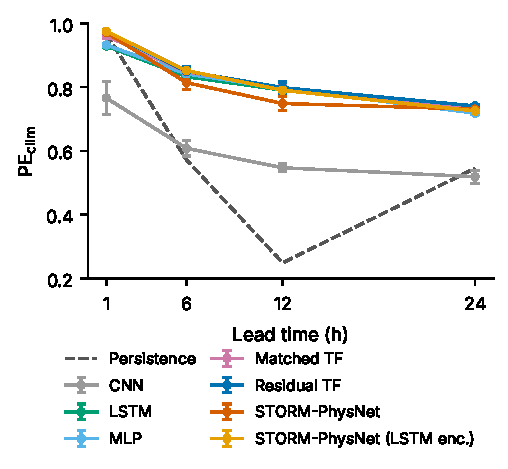
\includegraphics[width=\columnwidth]{figures/fig_horizon.pdf}
\caption{Test \(\PE_{\mathrm{clim}}\) against lead time (mean and standard deviation over ten seeds, averaged
over the three blocks). Dashed line: persistence, which recovers at 24\,h because of the daily cycle of GEO
flux.}
\label{fig:horizon}
\end{figure}

\begin{figure*}[!t]
\centering
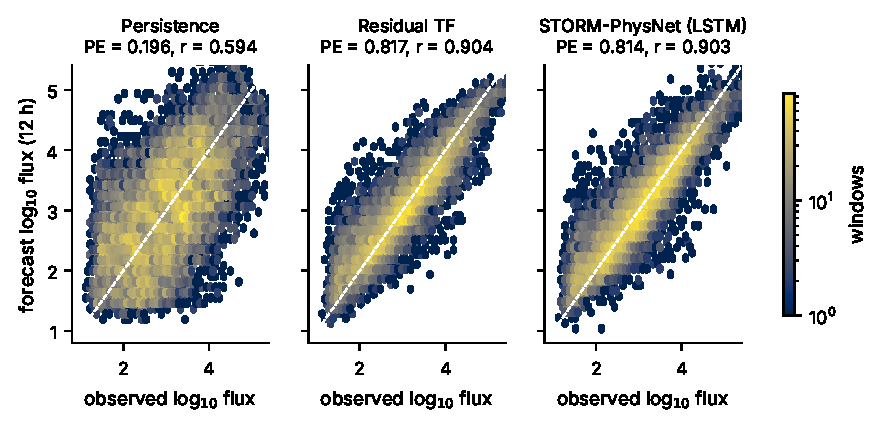
\includegraphics[width=\textwidth]{figures/fig_scatter.pdf}
\caption{12\,h forecasts against observations in block B (2015--2016), for persistence and the ten-seed mean
forecasts of two models. Colour: number of forecast windows per cell (logarithmic). Dashed line: equality.}
\label{fig:scatter}
\end{figure*}

\begin{table*}[!t]
\centering
\caption{Block A (strictly chronological test, Sep 2018--Mar 2020): $\mathrm{PE}_\mathrm{clim}$, mean over ten seeds.}
\label{tab:blockA}
\footnotesize
\setlength{\tabcolsep}{4pt}
\begin{adjustbox}{max width=\linewidth}
\begin{tabular}{lcccc}
\toprule
Model & 1\,h & 6\,h & 12\,h & 24\,h \\
\midrule
\multicolumn{5}{l}{\textit{Classical baselines}} \\
Ridge regression, residual & 0.976 & 0.835 & 0.796 & 0.767 \\
Gradient-boosted trees, residual & 0.978 & 0.848 & 0.815 & 0.762 \\
\multicolumn{5}{l}{\textit{Baselines}} \\
LSTM & 0.930 & 0.824 & 0.791 & 0.740 \\
LSTM, residual & 0.975 & 0.827 & 0.780 & 0.754 \\
\quad width 64 & 0.975 & 0.826 & 0.779 & 0.755 \\
\quad width 256 & 0.974 & 0.819 & 0.776 & 0.758 \\
MLP & 0.932 & 0.831 & 0.794 & 0.733 \\
CNN & 0.805 & 0.589 & 0.537 & 0.549 \\
\multicolumn{5}{l}{\textit{Transformer controls}} \\
Transformer (default size) & 0.957 & 0.833 & 0.797 & 0.756 \\
Transformer, matched & 0.966 & 0.830 & 0.793 & 0.756 \\
Transformer, FFN 256 & 0.966 & 0.840 & 0.795 & 0.756 \\
Residual Transformer & 0.975 & 0.844 & 0.808 & 0.760 \\
\quad + fixed average & 0.975 & 0.843 & 0.805 & 0.759 \\
Flux-only Transformer & 0.963 & 0.805 & 0.741 & 0.662 \\
\multicolumn{5}{l}{\textit{STORM-PhysNet and variants}} \\
STORM-PhysNet & 0.971 & 0.797 & 0.768 & 0.760 \\
\quad fixed average & 0.971 & 0.794 & 0.763 & 0.761 \\
\quad no delay & 0.973 & 0.810 & 0.768 & 0.760 \\
\quad no gate & 0.971 & 0.786 & 0.752 & 0.757 \\
\quad no physics loss & 0.973 & 0.808 & 0.778 & 0.761 \\
\quad physical-unit loss & 0.972 & 0.797 & 0.767 & 0.758 \\
\quad physical-unit loss from epoch 1 & 0.972 & 0.800 & 0.772 & 0.759 \\
\quad cathode--anode gate & 0.972 & 0.805 & 0.770 & 0.759 \\
\quad cathode--anode + spectral head & 0.971 & 0.799 & 0.763 & 0.759 \\
\quad radiotrophic gate & 0.972 & 0.802 & 0.770 & 0.759 \\
\quad LSTM encoder & 0.975 & 0.828 & 0.780 & 0.750 \\
\quad LSTM encoder, no gate & 0.976 & 0.830 & 0.783 & 0.750 \\
\quad LSTM encoder, no delay & 0.976 & 0.827 & 0.783 & 0.750 \\
\quad LSTM encoder, no physics loss & 0.976 & 0.827 & 0.782 & 0.747 \\
\quad LSTM encoder, physical-unit loss & 0.975 & 0.826 & 0.779 & 0.748 \\
\quad LSTM encoder, physical-unit loss from epoch 1 & 0.975 & 0.828 & 0.782 & 0.750 \\
\quad + magnetopause features & 0.973 & 0.808 & 0.776 & 0.761 \\
\bottomrule
\end{tabular}
\end{adjustbox}

\end{table*}


\subsection{What drives the skill}
\label{sec:attribution}
Table~\ref{tab:paired} and Fig.~\ref{fig:attribution} compare STORM-PhysNet with every other model. Four
findings stand out.

\emph{The persistence residual gives the 1\,h skill.} STORM-PhysNet beats the matched Transformer by 0.011 at
1\,h, but the residual Transformer, which has the residual and none of the physics components, matches it
(difference 0.001, not significant).

\emph{The solar-wind drivers give the longer-range skill.} Without them the matched Transformer loses 0.05 at
12\,h and 0.09 at 24\,h, but nothing at 1\,h.

\emph{The physics-inspired components do not change accuracy significantly.} Removing the delay stage or the
gate, replacing the learned delay with a fixed average, removing the physics loss, or replacing the gate with
either alternative gate changes no score by more than 0.011, and none of these differences is significant
(Fig.~\ref{fig:attribution}). The spectral head and the magnetopause features behave in the same way. The
learned delay averages \(\tau=1.36\)\,h and acts in practice as a short smoother.

\emph{The encoder matters.} Replacing the Transformer with an LSTM raises the 1\,h score to 0.975, the highest of
all 19 models (\(+0.003\) over the residual Transformer, paired \(p<0.001\)), and the 6 and 12\,h scores by 0.04
(Holm-adjusted \(p=0.04\) and 0.02 against STORM-PhysNet), while it loses 0.006 at 24\,h (not significant). It
also makes training far more reproducible: the standard deviation over seeds at 6 and 12\,h falls from
0.014--0.027 for the variants with a Transformer encoder to 0.004--0.005. Whether this gain comes from the LSTM
alone or from its combination with the residual, gate and loss is tested by the second campaign \pend.

\begin{table*}[!t]
\centering
\caption{Difference in $\mathrm{PE}_\mathrm{clim}$, STORM-PhysNet minus each model (positive: STORM-PhysNet better).}
\label{tab:paired}
\footnotesize
\setlength{\tabcolsep}{4pt}
\begin{adjustbox}{max width=\linewidth}
\begin{tabular}{lcccc}
\toprule
STORM-PhysNet minus & 1\,h & 6\,h & 12\,h & 24\,h \\
\midrule
Ridge regression, residual & -0.0041$^{*}$ & -0.0336 & -0.0454$^{*}$ & -0.0140$^{*}$ \\
Gradient-boosted trees, residual & \pend{} & \pend{} & \pend{} & \pend{} \\
LSTM & +0.0424$^{*}$ & -0.0187 & -0.0420$^{*}$ & +0.0054 \\
LSTM, residual & -0.0023 & -0.0352 & -0.0404$^{*}$ & -0.0008 \\
LSTM, residual, width 64 & \pend{} & \pend{} & \pend{} & \pend{} \\
LSTM, residual, width 256 & \pend{} & \pend{} & \pend{} & \pend{} \\
MLP & +0.0393$^{*}$ & -0.0277 & -0.0471$^{*}$ & +0.0127$^{*}$ \\
CNN & +0.2056$^{*}$ & +0.2058$^{*}$ & +0.2015$^{*}$ & +0.2118$^{*}$ \\
Transformer (default size) & +0.0132$^{*}$ & -0.0363 & -0.0531$^{*}$ & -0.0023 \\
Transformer, matched & +0.0107 & -0.0338 & -0.0486$^{*}$ & -0.0058 \\
Transformer, FFN 256 & +0.0114$^{*}$ & -0.0346 & -0.0501$^{*}$ & -0.0063 \\
Residual Transformer & -0.0009 & -0.0357$^{*}$ & -0.0496$^{*}$ & -0.0097 \\
Residual TF + fixed average & -0.0009 & -0.0334 & -0.0463$^{*}$ & -0.0067 \\
Flux-only Transformer & +0.0093$^{*}$ & -0.0090 & +0.0020 & +0.0846$^{*}$ \\
STORM-PhysNet, fixed average & +0.0005 & +0.0027 & +0.0038 & -0.0018 \\
STORM-PhysNet, no delay & +0.0006 & +0.0000 & +0.0004 & -0.0045 \\
STORM-PhysNet, no gate & -0.0006 & -0.0035 & -0.0056 & -0.0010 \\
STORM-PhysNet, no physics loss & -0.0011 & -0.0102 & -0.0100 & +0.0014 \\
STORM-PhysNet, physical-unit loss & \pend{} & \pend{} & \pend{} & \pend{} \\
STORM-PhysNet, cathode--anode gate & -0.0006 & -0.0104 & -0.0068 & +0.0007 \\
STORM-PhysNet, cathode--anode + spectral head & +0.0004 & -0.0021 & -0.0040 & -0.0041 \\
STORM-PhysNet, radiotrophic gate & +0.0003 & +0.0067 & +0.0029 & -0.0015 \\
STORM-PhysNet, LSTM encoder & -0.0036 & -0.0378 & -0.0417$^{*}$ & +0.0059 \\
STORM-PhysNet, LSTM encoder, no gate & -0.0032 & -0.0352$^{*}$ & -0.0386$^{*}$ & +0.0051 \\
STORM-PhysNet, LSTM encoder, no delay & -0.0033 & -0.0362$^{*}$ & -0.0419$^{*}$ & +0.0025 \\
STORM-PhysNet, LSTM encoder, no physics loss & -0.0032 & -0.0336 & -0.0367$^{*}$ & +0.0061 \\
STORM-PhysNet, LSTM encoder, physical-unit loss & \pend{} & \pend{} & \pend{} & \pend{} \\
STORM-PhysNet, + magnetopause features & -0.0009 & -0.0074 & -0.0064 & +0.0009 \\
\bottomrule
\end{tabular}
\end{adjustbox}

\par\vspace{0.5ex}{\footnotesize\raggedright Paired $t$-test on the ten seed means (each averaged over blocks); $^{*}$ Holm-adjusted $p<0.05$ over all comparisons in the table.\par}
\end{table*}


\begin{figure*}[!t]
\centering
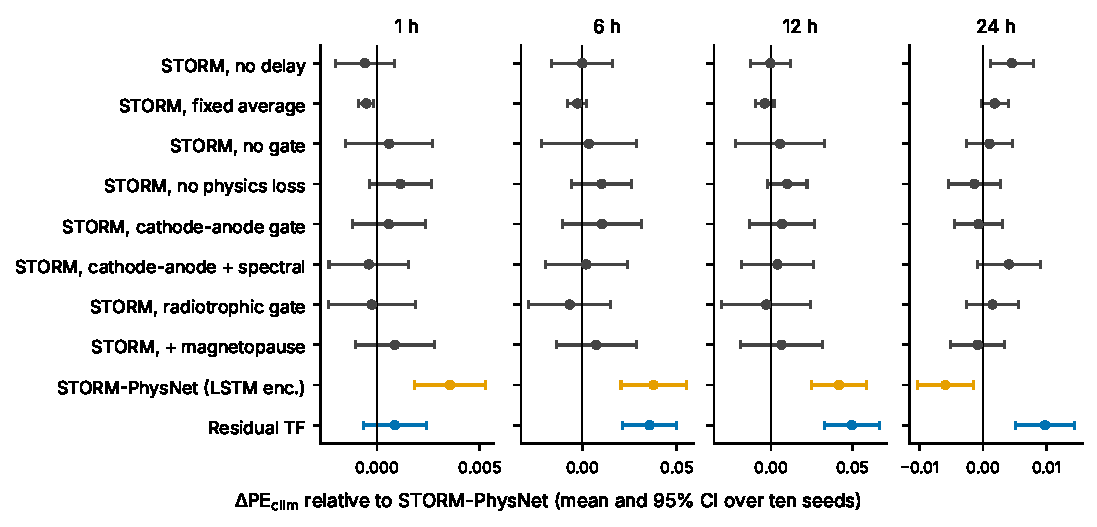
\includegraphics[width=\textwidth]{figures/fig_attribution.pdf}
\caption{Change in \(\PE_{\mathrm{clim}}\) from STORM-PhysNet to each variant and to the residual Transformer
(mean and 95\% confidence interval over ten seeds, each averaged over the three blocks). Intervals that include
zero mean no detectable effect. Note the different horizontal scales.}
\label{fig:attribution}
\end{figure*}

\subsection{Storm time and alerts}
\label{sec:storm}
At storm time (Table~\ref{tab:storm}) every model has a lower RMSE than persistence at 6--24\,h. The lowest
storm-time RMSE is reached by the LSTM variant of STORM-PhysNet at 6\,h (0.61), by the MLP at 12\,h (0.69) and by
the matched Transformer at 24\,h (0.76); the original STORM-PhysNet is 0.04--0.09 higher. At 1\,h the residual
models are best (0.28). For the 1000\,pfu alert, the residual models reach an HSS of 0.92--0.93 at 1\,h; at 6 and
12\,h the best models reach 0.78--0.79 and 0.74--0.75, against 0.74 and 0.71 for STORM-PhysNet and 0.61 and 0.45
for persistence.

Fig.~\ref{fig:case2015} shows the storm of 17 March 2015, the strongest of solar cycle 24. The flux was low and
mostly unobserved during the main phase, then rose by more than two orders of magnitude on 18--19 March and
stayed near or above the alert level until 28 March. At 12\,h, the models follow the rise within hours of its
appearance in the input, earlier than persistence; none forecasts the onset before the flux begins to rise.
At 24\,h the models already forecast the enhanced level on 19--20 March, when persistence still shows the
pre-storm level, but they miss the dip of 22--23 March by more than one order of magnitude and afterwards
largely follow the daily cycle, which shows the limit of a one-day forecast from these inputs.

\begin{table*}[!t]
\centering
\caption{Storm-time RMSE (log$_{10}$ flux; Dst $\le -50$\,nT at the target hour) and Heidke skill score for exceeding 1000\,pfu.}
\label{tab:storm}
\footnotesize
\setlength{\tabcolsep}{4pt}
\begin{adjustbox}{max width=\linewidth}
\begin{tabular}{lcccccccc}
\toprule
 & \multicolumn{4}{c}{Storm-time RMSE} & \multicolumn{4}{c}{Alert HSS} \\
Model & 1\,h & 6\,h & 12\,h & 24\,h & 1\,h & 6\,h & 12\,h & 24\,h \\
\midrule
Persistence & 0.290 & 0.838 & 1.125 & 1.053 & 0.907 & 0.608 & 0.452 & 0.658 \\
Ridge regression, residual & 0.268 & 0.623 & 0.701 & 0.720 & 0.929 & 0.783 & 0.735 & 0.707 \\
Gradient-boosted trees, residual & 0.258 & 0.583 & 0.667 & 0.763 & 0.934 & 0.797 & 0.765 & 0.717 \\
LSTM & 0.400 & 0.649 & 0.749 & 0.810 & 0.861 & 0.772 & 0.746 & 0.707 \\
LSTM, residual & 0.288 & 0.619 & 0.714 & 0.799 & 0.927 & 0.787 & 0.749 & 0.717 \\
\quad width 64 & 0.286 & 0.629 & 0.726 & 0.796 & 0.927 & 0.784 & 0.745 & 0.717 \\
\quad width 256 & 0.291 & 0.648 & 0.753 & 0.805 & 0.927 & 0.781 & 0.740 & 0.715 \\
MLP & 0.378 & 0.627 & 0.692 & 0.814 & 0.855 & 0.767 & 0.730 & 0.690 \\
CNN & 0.562 & 0.823 & 0.917 & 1.014 & 0.720 & 0.599 & 0.560 & 0.558 \\
Transformer (default size) & 0.317 & 0.622 & 0.708 & 0.777 & 0.896 & 0.780 & 0.750 & 0.716 \\
Transformer, matched & 0.310 & 0.614 & 0.714 & 0.762 & 0.901 & 0.782 & 0.748 & 0.715 \\
Transformer, FFN 256 & 0.313 & 0.627 & 0.726 & 0.776 & 0.903 & 0.786 & 0.753 & 0.713 \\
Residual Transformer & 0.282 & 0.630 & 0.736 & 0.773 & 0.923 & 0.781 & 0.744 & 0.715 \\
\quad + fixed average & 0.281 & 0.644 & 0.745 & 0.777 & 0.922 & 0.781 & 0.742 & 0.713 \\
Flux-only Transformer & 0.299 & 0.650 & 0.739 & 0.869 & 0.903 & 0.766 & 0.715 & 0.656 \\
STORM-PhysNet & 0.282 & 0.678 & 0.784 & 0.798 & 0.918 & 0.744 & 0.708 & 0.713 \\
\quad fixed average & 0.283 & 0.673 & 0.777 & 0.799 & 0.917 & 0.743 & 0.704 & 0.715 \\
\quad no delay & 0.282 & 0.661 & 0.771 & 0.797 & 0.918 & 0.746 & 0.710 & 0.717 \\
\quad no gate & 0.283 & 0.671 & 0.778 & 0.797 & 0.919 & 0.748 & 0.712 & 0.714 \\
\quad no physics loss & 0.281 & 0.677 & 0.774 & 0.800 & 0.921 & 0.754 & 0.717 & 0.711 \\
\quad physical-unit loss & 0.282 & 0.673 & 0.782 & 0.803 & 0.918 & 0.745 & 0.710 & 0.713 \\
\quad cathode--anode gate & 0.283 & 0.680 & 0.796 & 0.802 & 0.920 & 0.756 & 0.714 & 0.711 \\
\quad cathode--anode + spectral head & 0.286 & 0.681 & 0.791 & 0.796 & 0.918 & 0.750 & 0.714 & 0.713 \\
\quad radiotrophic gate & 0.282 & 0.688 & 0.794 & 0.795 & 0.918 & 0.743 & 0.712 & 0.716 \\
\quad LSTM encoder & 0.279 & 0.612 & 0.713 & 0.793 & 0.930 & 0.790 & 0.748 & 0.713 \\
\quad LSTM encoder, no gate & 0.282 & 0.621 & 0.724 & 0.799 & 0.928 & 0.786 & 0.746 & 0.715 \\
\quad LSTM encoder, no delay & 0.281 & 0.623 & 0.716 & 0.793 & 0.929 & 0.784 & 0.745 & 0.715 \\
\quad LSTM encoder, no physics loss & 0.281 & 0.620 & 0.712 & 0.798 & 0.928 & 0.785 & 0.744 & 0.714 \\
\quad LSTM encoder, physical-unit loss & 0.282 & 0.611 & 0.717 & 0.789 & 0.928 & 0.785 & 0.745 & 0.711 \\
\quad + magnetopause features & 0.282 & 0.677 & 0.777 & 0.801 & 0.921 & 0.753 & 0.714 & 0.710 \\
\bottomrule
\end{tabular}
\end{adjustbox}

\par\vspace{0.5ex}{\footnotesize\raggedright Seed means over the three blocks. Lower RMSE and higher HSS are better.\par}
\end{table*}


\begin{figure*}[!t]
\centering
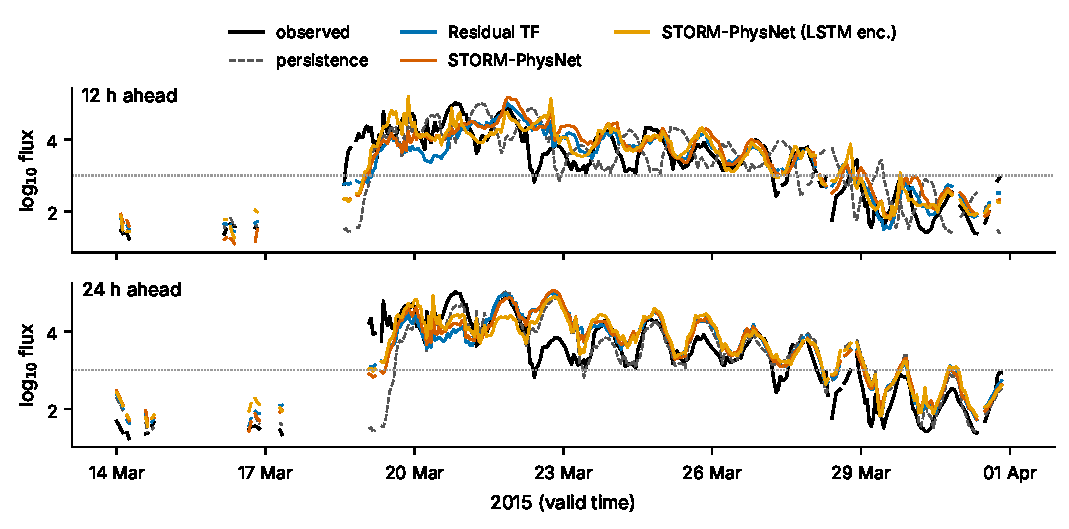
\includegraphics[width=\textwidth]{figures/fig_case_2015.pdf}
\caption{GOES-15 flux during the March 2015 storm (block B) and the 12\,h (top) and 24\,h (bottom) forecasts,
plotted at the time they are valid for (ten-seed means). Gaps are hours without observations. Dotted line:
1000\,pfu alert level.}
\label{fig:case2015}
\end{figure*}

\subsection{Robustness to degraded inputs}
\label{sec:robust}
Noise separates the models more than clean data do (Table~\ref{tab:probes}, Fig.~\ref{fig:noise}). The LSTM
variant of STORM-PhysNet is the most robust model at every lead time: at \(\sigma=1\) it keeps 0.736 at 12\,h,
against 0.711 for the MLP, 0.680 for the residual Transformer with the fixed average, 0.606 for the plain
residual Transformer and 0.56--0.58 for the Transformer variants of STORM-PhysNet; at \(\sigma=2\) it keeps
0.603, against at most 0.465 for any other model. The Transformer variants of STORM-PhysNet are robust at 1 and
24\,h (0.968 and about 0.69 at \(\sigma=1\)) but not at 6--12\,h. The CNN fails under noise. When driver data are
missing for the last 24\,h or entirely, every model falls back towards its skill from the flux history alone;
the LSTM variant again keeps the most (12\,h: 0.679 and 0.681, against 0.61--0.63 for the next-best models).
Kp and Dst arriving three hours late change no model by more than 0.004.

\begin{table*}[!t]
\centering
\caption{Robustness probes: 12\,h $\mathrm{PE}_\mathrm{clim}$ with degraded inputs (seed means over blocks).}
\label{tab:probes}
\footnotesize
\setlength{\tabcolsep}{4pt}
\begin{adjustbox}{max width=\linewidth}
\begin{tabular}{lcccccc}
\toprule
Model & $\sigma=0.5$ & $\sigma=1$ & $\sigma=2$ & 24\,h outage & no drivers & Kp/Dst 3\,h late \\
\midrule
Ridge regression, residual & 0.744 & 0.592 & -0.034 & 0.671 & 0.666 & 0.793 \\
Gradient-boosted trees, residual & 0.789 & 0.738 & 0.662 & 0.646 & 0.602 & 0.813 \\
LSTM, residual & 0.772 & 0.724 & 0.574 & 0.666 & 0.677 & 0.786 \\
\quad width 64 & 0.767 & 0.713 & 0.555 & 0.663 & 0.674 & 0.784 \\
\quad width 256 & 0.764 & 0.713 & 0.564 & 0.653 & 0.662 & 0.777 \\
\quad training protocol B & 0.772 & 0.721 & 0.566 & 0.662 & 0.675 & 0.786 \\
MLP & 0.774 & 0.711 & 0.465 & 0.625 & 0.620 & 0.792 \\
CNN & 0.033 & -2.232 & -12.587 & 0.390 & -0.290 & 0.545 \\
Transformer (default size) & 0.767 & 0.656 & 0.323 & 0.580 & 0.583 & 0.799 \\
Transformer, matched & 0.765 & 0.660 & 0.330 & 0.589 & 0.609 & 0.795 \\
Transformer, FFN 256 & 0.761 & 0.646 & 0.291 & 0.582 & 0.621 & 0.797 \\
Residual Transformer & 0.746 & 0.606 & 0.258 & 0.612 & 0.604 & 0.797 \\
\quad training protocol B & 0.764 & 0.623 & 0.246 & 0.631 & 0.621 & 0.808 \\
\quad + fixed average & 0.764 & 0.680 & 0.431 & 0.612 & 0.603 & 0.794 \\
STORM-PhysNet & 0.696 & 0.563 & 0.289 & 0.568 & 0.537 & 0.746 \\
\quad training protocol B & 0.758 & 0.645 & 0.377 & 0.633 & 0.658 & 0.792 \\
\quad fixed average & 0.696 & 0.567 & 0.292 & 0.558 & 0.535 & 0.743 \\
\quad no physics loss & 0.707 & 0.577 & 0.308 & 0.583 & 0.559 & 0.756 \\
\quad physical-unit loss & 0.698 & 0.568 & 0.295 & 0.572 & 0.538 & 0.747 \\
\quad physical-unit loss from epoch 1 & 0.702 & 0.572 & 0.301 & 0.574 & 0.554 & 0.751 \\
\quad cathode--anode gate & 0.705 & 0.580 & 0.326 & 0.571 & 0.507 & 0.754 \\
\quad cathode--anode + spectral head & 0.701 & 0.570 & 0.286 & 0.558 & 0.515 & 0.752 \\
\quad radiotrophic gate & 0.693 & 0.563 & 0.299 & 0.560 & 0.480 & 0.743 \\
\quad LSTM encoder & 0.777 & 0.736 & 0.603 & 0.679 & 0.681 & 0.788 \\
\quad LSTM encoder, training protocol B & 0.773 & 0.731 & 0.598 & 0.677 & 0.689 & 0.784 \\
\quad LSTM encoder, no gate & 0.775 & 0.738 & 0.621 & 0.677 & 0.666 & 0.785 \\
\quad LSTM encoder, no delay & 0.775 & 0.726 & 0.563 & 0.668 & 0.677 & 0.788 \\
\quad LSTM encoder, no physics loss & 0.771 & 0.728 & 0.591 & 0.673 & 0.678 & 0.783 \\
\quad LSTM encoder, physical-unit loss & 0.775 & 0.733 & 0.599 & 0.676 & 0.684 & 0.786 \\
\quad LSTM encoder, physical-unit loss from epoch 1 & 0.774 & 0.734 & 0.603 & 0.677 & 0.683 & 0.785 \\
\quad + magnetopause features & 0.703 & 0.573 & 0.311 & 0.576 & 0.554 & 0.753 \\
\bottomrule
\end{tabular}
\end{adjustbox}

\par\vspace{0.5ex}{\footnotesize\raggedright Noise: Gaussian noise of standard deviation $\sigma$ (in units of each standardised channel) on the 16 continuous auxiliary channels; the flux history and the observed-hour mask are unchanged. Outage: driver channels held at their last value for the final 24 input hours. No drivers: driver channels at their training mean for the whole input. Clean values are in Table~\ref{tab:main}.\par}
\end{table*}


\begin{figure*}[!t]
\centering
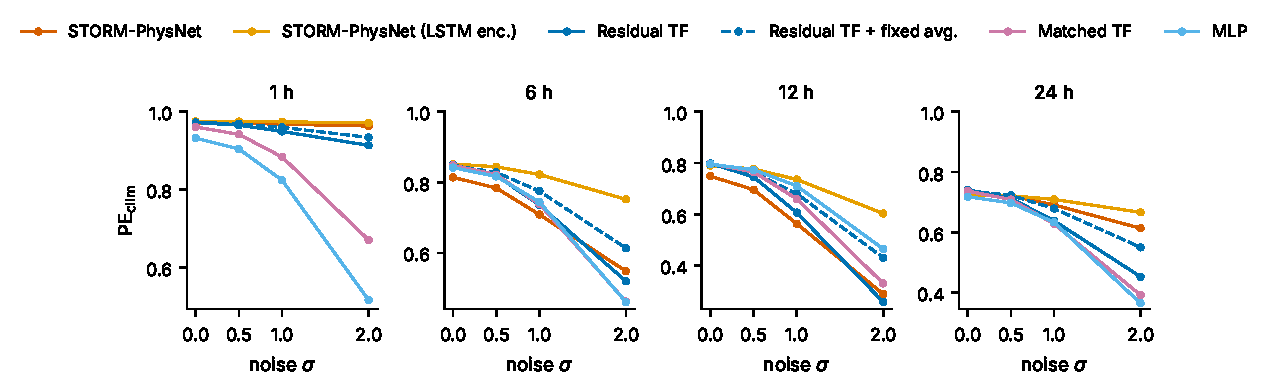
\includegraphics[width=\textwidth]{figures/fig_noise.pdf}
\caption{Test \(\PE_{\mathrm{clim}}\) against the standard deviation of the noise added to the inputs, for each
lead time.}
\label{fig:noise}
\end{figure*}

\subsection{Uncertainty}
\label{sec:calib}
The uncertainty predicted by STORM-PhysNet is close to calibrated (Table~\ref{tab:calib},
Fig.~\ref{fig:calib}): 67--72\% of the observations fall inside \(\hat y\pm\hat\sigma\) (nominally 68\%), and
91--94\% inside \(\hat y\pm1.96\hat\sigma\) (nominally 95\%), so the wider interval is slightly too narrow at
6--24\,h. The LSTM variant is similar but a little over-confident at 6 and 12\,h (65\% and 90\%). Its Gaussian
CRPS is the lowest of all variants at 1--12\,h (0.060, 0.161 and 0.198, against 0.066, 0.183 and 0.219 for
STORM-PhysNet). For models that predict no uncertainty, the ten trained seeds form an ensemble; averaging them
raises PE by 0.01--0.04 at 6--12\,h (residual Transformer at 6\,h: 0.850 to 0.871), and the ensemble CRPS of the
residual Transformer (0.067, 0.167 and 0.198) is close to that of the LSTM variant's single-model uncertainty.

\begin{table*}[!t]
\centering
\caption{Coverage of the predicted $1\sigma$ / $1.96\sigma$ intervals (nominal 0.68 / 0.95).}
\label{tab:calib}
\footnotesize
\setlength{\tabcolsep}{4pt}
\begin{adjustbox}{max width=\linewidth}
\begin{tabular}{lcccc}
\toprule
Model & 1\,h & 6\,h & 12\,h & 24\,h \\
\midrule
STORM-PhysNet & 0.72 / 0.94 & 0.67 / 0.92 & 0.69 / 0.93 & 0.70 / 0.91 \\
\quad fixed average & 0.71 / 0.94 & 0.67 / 0.92 & 0.69 / 0.93 & 0.70 / 0.91 \\
\quad no delay & 0.70 / 0.94 & 0.66 / 0.92 & 0.69 / 0.93 & 0.71 / 0.92 \\
\quad no gate & 0.70 / 0.94 & 0.66 / 0.91 & 0.68 / 0.92 & 0.69 / 0.90 \\
\quad no physics loss & 0.71 / 0.94 & 0.65 / 0.91 & 0.68 / 0.92 & 0.68 / 0.90 \\
\quad physics loss in physical units & \pend{} & \pend{} & \pend{} & \pend{} \\
\quad cathode--anode gate & 0.71 / 0.94 & 0.66 / 0.91 & 0.69 / 0.92 & 0.70 / 0.91 \\
\quad cathode--anode + spectral head & 0.71 / 0.94 & 0.67 / 0.92 & 0.69 / 0.93 & 0.71 / 0.92 \\
\quad radiotrophic gate & 0.71 / 0.94 & 0.66 / 0.92 & 0.70 / 0.93 & 0.70 / 0.91 \\
\quad LSTM encoder & 0.75 / 0.94 & 0.65 / 0.90 & 0.65 / 0.90 & 0.69 / 0.91 \\
\quad LSTM encoder, no gate & 0.74 / 0.94 & 0.66 / 0.90 & 0.67 / 0.91 & 0.71 / 0.92 \\
\quad LSTM encoder, no delay & 0.74 / 0.94 & 0.65 / 0.90 & 0.66 / 0.91 & 0.72 / 0.92 \\
\quad LSTM encoder, no physics loss & 0.75 / 0.95 & 0.65 / 0.90 & 0.66 / 0.90 & 0.71 / 0.91 \\
\quad LSTM encoder, physics loss in physical units & \pend{} & \pend{} & \pend{} & \pend{} \\
\quad + magnetopause features & 0.73 / 0.95 & 0.66 / 0.92 & 0.69 / 0.92 & 0.70 / 0.91 \\
\bottomrule
\end{tabular}
\end{adjustbox}

\par\vspace{0.5ex}{\footnotesize\raggedright Fraction of test targets inside $\hat y\pm\hat\sigma$ and $\hat y\pm1.96\hat\sigma$, averaged over seeds and blocks.\par}
\end{table*}


\begin{figure}[!t]
\centering
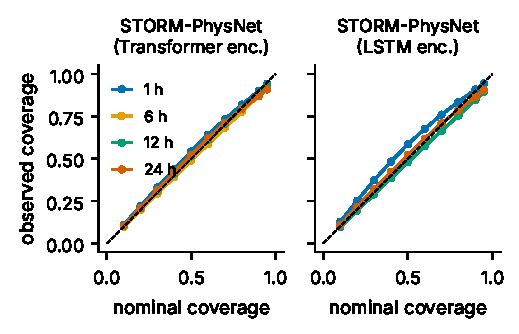
\includegraphics[width=\columnwidth]{figures/fig_calibration.pdf}
\caption{Fraction of observations inside the central interval of the predicted Gaussian against the nominal
fraction, per lead time. A calibrated forecast lies on the dashed line; points below it are over-confident.}
\label{fig:calib}
\end{figure}

\subsection{Transfer to other satellites}
\label{sec:transfer}
Table~\ref{tab:transfer} and Fig.~\ref{fig:transfer} give the 12\,h skill on the other satellites.

\emph{GOES-16} (different longitude, flux a factor of two lower). Without retraining, the residual models keep
part of their skill and the LSTM variant keeps the most (0.371; STORM-PhysNet 0.306, residual Transformer
0.214; persistence 0.201). Every model that forecasts the flux level directly falls far below persistence
(from 0.010 for the default Transformer to \(-0.50\) for the CNN), because it forecasts the GOES-15 level.
Predicting changes rather than levels is therefore what survives the offset. No model beats persistence
zero-shot at 24\,h. With all weights fine-tuned, the models reach 0.66--0.69, and training from scratch on
GOES-16 alone is almost as good, because its record is long.

\emph{GOES-18} (same longitude as GOES-15). Zero-shot skill is much higher (0.50--0.64 for all but the CNN), and
the LSTM variant again leads (0.640). After fine-tuning the models reach 0.76--0.80. Persistence is negative at
12\,h (\(-0.34\)), which shows how strong the daily cycle is at this position.

\emph{GSAT-19 GRASP} (48\(^\circ\)E, no driver data). Zero-shot, the residual Transformer transfers best
(0.737), followed by the Transformer with an FFN width of 256 (0.697) and the LSTM variant (0.687); after full
fine-tuning the models reach 0.78--0.81.

Fig.~\ref{fig:case2024} shows GOES-16 during the storm of May 2024. GOES-16 recorded a moderate enhancement that
reached about the alert level on 15--16 May. On 13 May, the first day with data after the storm onset, the
zero-shot matched Transformer forecast up to \(10^{4.2}\)\,pfu, about two orders of magnitude above the
observation, and the zero-shot LSTM variant up to \(10^{3.8}\)\,pfu; from 14 May the LSTM variant followed the
observation, while the matched Transformer stayed about half an order of magnitude too high. The residual
Transformer fine-tuned on GOES-16 was closest throughout. Fine-tuning on local data is therefore needed before a
forecast can be trusted at a new position.

\begin{table*}[!t]
\centering
\caption{Cross-satellite transfer from the block-A GOES-15 models: 12\,h $\mathrm{PE}_\mathrm{clim}$, mean over folds and ten seeds.}
\label{tab:transfer}
\footnotesize
\setlength{\tabcolsep}{4pt}
\begin{adjustbox}{max width=\linewidth}
\begin{tabular}{lcccccccccccc}
\toprule
 & \multicolumn{4}{c}{GOES-16 (75\textdegree W)} & \multicolumn{4}{c}{GOES-18 (137\textdegree W)} & \multicolumn{4}{c}{GSAT-19 GRASP (48\textdegree E)} \\
\cmidrule(lr){2-5}\cmidrule(lr){6-9}\cmidrule(lr){10-13}
Model & zero & heads & full & scr. & zero & heads & full & scr. & zero & heads & full & scr. \\
\midrule
Persistence & \multicolumn{4}{c}{0.201} & \multicolumn{4}{c}{-0.336} & \multicolumn{4}{c}{0.129} \\
Ridge regression, residual & 0.489 & -- & -- & -- & 0.699 & -- & -- & -- & 0.552 & -- & -- & -- \\
Gradient-boosted trees, residual & 0.490 & -- & -- & -- & 0.699 & -- & -- & -- & 0.656 & -- & -- & -- \\
LSTM, residual & 0.455 & 0.628 & 0.680 & -- & 0.661 & 0.754 & 0.772 & -- & 0.673 & 0.751 & 0.785 & -- \\
\quad width 64 & \pend{} & \pend{} & \pend{} & \pend{} & \pend{} & \pend{} & \pend{} & \pend{} & \pend{} & \pend{} & \pend{} & \pend{} \\
\quad width 256 & \pend{} & \pend{} & \pend{} & \pend{} & \pend{} & \pend{} & \pend{} & \pend{} & \pend{} & \pend{} & \pend{} & \pend{} \\
MLP & -0.065 & -- & -- & -- & 0.505 & -- & -- & -- & 0.656 & -- & -- & -- \\
CNN & -0.497 & -- & -- & -- & 0.216 & -- & -- & -- & 0.297 & -- & -- & -- \\
Transformer (default size) & 0.010 & 0.617 & 0.682 & -- & 0.532 & 0.783 & 0.798 & -- & 0.646 & 0.762 & 0.803 & -- \\
Transformer, matched & -0.053 & 0.624 & 0.689 & 0.682 & 0.496 & 0.787 & 0.797 & 0.774 & 0.664 & 0.768 & 0.802 & 0.802 \\
Transformer, FFN 256 & 0.003 & -- & -- & -- & 0.523 & -- & -- & -- & 0.697 & -- & -- & -- \\
Residual Transformer & 0.214 & 0.660 & 0.693 & 0.692 & 0.604 & 0.778 & 0.792 & 0.776 & 0.737 & 0.772 & 0.808 & 0.805 \\
STORM-PhysNet & 0.306 & 0.630 & 0.672 & 0.669 & 0.575 & 0.718 & 0.773 & 0.754 & 0.634 & 0.741 & 0.791 & 0.795 \\
\quad no physics loss & 0.328 & 0.640 & 0.680 & -- & 0.608 & 0.730 & 0.777 & -- & 0.630 & 0.743 & 0.795 & -- \\
\quad physical-unit loss & \pend{} & \pend{} & \pend{} & \pend{} & \pend{} & \pend{} & \pend{} & \pend{} & \pend{} & \pend{} & \pend{} & \pend{} \\
\quad cathode--anode gate & 0.325 & 0.631 & 0.678 & -- & 0.581 & 0.724 & 0.777 & -- & 0.648 & 0.746 & 0.799 & -- \\
\quad cathode--anode + spectral head & 0.301 & 0.636 & 0.674 & -- & 0.590 & 0.726 & 0.778 & -- & 0.656 & 0.740 & 0.798 & -- \\
\quad radiotrophic gate & 0.319 & 0.637 & 0.675 & -- & 0.599 & 0.726 & 0.769 & -- & 0.617 & 0.747 & 0.797 & -- \\
\quad LSTM encoder & 0.371 & 0.640 & 0.659 & -- & 0.640 & 0.748 & 0.759 & -- & 0.687 & 0.751 & 0.784 & -- \\
\quad LSTM encoder, no gate & 0.429 & -- & -- & -- & 0.652 & -- & -- & -- & 0.707 & -- & -- & -- \\
\quad LSTM encoder, no delay & 0.381 & -- & -- & -- & 0.636 & -- & -- & -- & 0.689 & -- & -- & -- \\
\quad LSTM encoder, no physics loss & 0.386 & -- & -- & -- & 0.648 & -- & -- & -- & 0.696 & -- & -- & -- \\
\quad LSTM encoder, physical-unit loss & \pend{} & \pend{} & \pend{} & \pend{} & \pend{} & \pend{} & \pend{} & \pend{} & \pend{} & \pend{} & \pend{} & \pend{} \\
\quad + magnetopause features & 0.293 & 0.631 & 0.675 & -- & 0.584 & 0.722 & 0.774 & -- & 0.635 & 0.746 & 0.796 & -- \\
\bottomrule
\end{tabular}
\end{adjustbox}

\par\vspace{0.5ex}{\footnotesize\raggedright Zero: zero-shot, no retraining. Heads: encoder frozen, output layers retrained. Full: all weights fine-tuned. Scr.: trained from scratch on the target satellite only. ``--'': not run (zero-shot only for these models).\par}
\end{table*}


\begin{figure*}[!t]
\centering
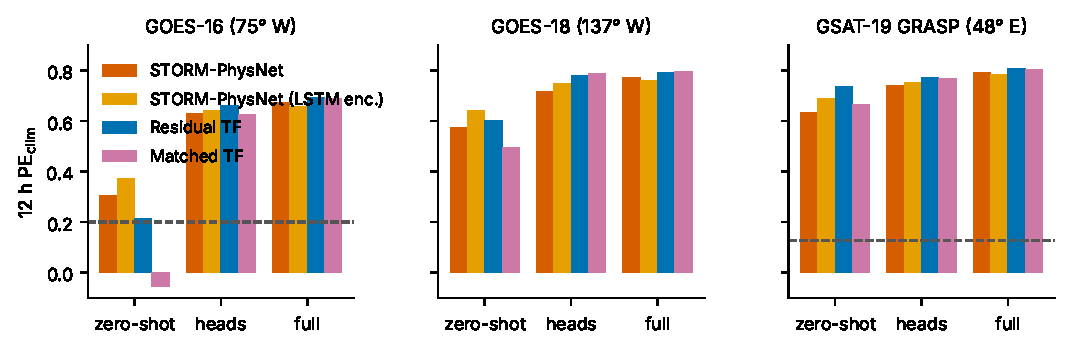
\includegraphics[width=\textwidth]{figures/fig_transfer.pdf}
\caption{12\,h \(\PE_{\mathrm{clim}}\) on each target satellite for zero-shot use, retrained heads and full
fine-tuning (means over folds and ten seeds). Dashed lines: persistence on that satellite.}
\label{fig:transfer}
\end{figure*}

\begin{figure*}[!t]
\centering
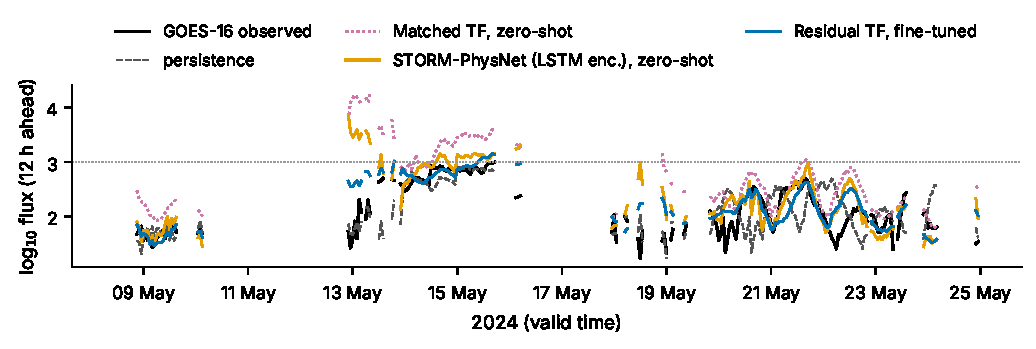
\includegraphics[width=\textwidth]{figures/fig_case_2024.pdf}
\caption{GOES-16 flux during the May 2024 storm (fold F2) and 12\,h forecasts at their valid times (ten-seed
means): zero-shot models trained on GOES-15 and the residual Transformer fine-tuned on GOES-16. Gaps are hours
without observations. Dotted line: 1000\,pfu alert level.}
\label{fig:case2024}
\end{figure*}

%% =====================================================================================================
\section{Discussion}
\label{sec:discussion}
%% =====================================================================================================
\subsection{Which model should an operator use?}
On clean GOES-15 data, three model types perform about equally well at 6--24\,h: the residual Transformer, the
Transformers without a residual, and the LSTM variant of STORM-PhysNet. The LSTM variant is the best choice
overall: it is best at 1\,h, ties at 6\,h, is the most robust when inputs are noisy or missing, transfers best
without retraining to the two GOES satellites, and gives the most reproducible training. Its cost is a small
loss at 24\,h (0.016 below the residual Transformer). If a new satellite has a year or more of data,
fine-tuning any of the strong models gives similar skill, and the choice of architecture matters little.

\subsection{Why do the physics components not help?}
The learned delay settles near a short average because the OMNI data are already propagated to the bow shock;
the remaining timing error is smaller than the hourly resolution. The gate and the physics loss act mainly on
the 1\,h forecast, where persistence already explains most of the variance, and the information they encode,
southward \(B_z\) and energy input, is also present in the driver channels that every model sees. The
alternative gates, the spectral head and the magnetopause features add the same information in other forms,
and also leave the skill unchanged. Physical knowledge helped in this study through the choice of target (a
change from persistence) and of inputs, not through specialised layers or loss terms.

\subsection{Why does the LSTM encoder help?}
With 72 hourly inputs and a target that depends mostly on the recent past, an encoder that reads the window in
time order with a memory may suit the problem better than one in which every hour attends to every other. The
lower spread over seeds also suggests that the Transformer variants are harder to train with the combined loss.
The second campaign separates the effect of the LSTM from that of the residual and of the other STORM-PhysNet
components \pend.

\subsection{Longitude and calibration}
GOES-16 sits at 75\(^\circ\)W, where geostationary orbit lies at a higher magnetic latitude than at
135\(^\circ\)W and crosses field lines that reach farther out; together with differences between the
instruments, this plausibly explains its lower flux. A forecast trained at one longitude and applied at another
should therefore predict changes rather than levels, or be recalibrated with local data. This matters for Indian
geostationary satellites, which no GOES satellite monitors.

\subsection{Limitations}
(1) The GOES-15 test periods cover solar cycle 24; GOES-16 and GOES-18 extend the evaluation into cycle 25 only
in the transfer experiments. (2) Blocks B and C are blocked cross-validation; block A is the only strictly
chronological GOES-15 test, and it contains few storms. (3) The models are not compared with NOAA's operational
forecast, whose past forecasts are not publicly archived. (4) The GRASP record is short (14 months) and is used
without driver inputs. (5) We use one GOES-16/18 telescope and no cross-calibration between satellites. (6) The
study is an offline evaluation, not an operational trial.

%% =====================================================================================================
\section{Conclusions}
\label{sec:conclusion}
%% =====================================================================================================
Under a protocol that prevents information leakage, with ten seeds on three test periods, forecasting the
change from persistence explains the 1\,h skill of forecasts of relativistic electrons at geostationary orbit,
and solar-wind inputs explain the 6--24\,h skill. A learned solar-wind delay, a \(B_z\)-conditioned gate, a
physics-informed loss, two alternative gates, a spectral head and magnetopause features do not change the
accuracy significantly. The encoder matters more: with an LSTM encoder, the physics-guided model is the most
accurate at 1\,h, the most robust to noisy and missing inputs, and the best at transferring without retraining
to GOES-16 and GOES-18. Models that forecast the flux level directly fail on a satellite whose flux differs by a
factor of two, while models that forecast changes keep part of their skill, and fine-tuning on local data
brings all strong models to similar skill on GOES-16, GOES-18 and GSAT-19.

%% =====================================================================================================
\section*{Data and code availability}
The code, configurations, data pipeline, processed GOES-16/18 and OMNI files and all predictions are available
at \url{https://github.com/bnsama29-cloud/STORM-PhysNet-L2}. GOES-15 data are from NOAA, accessed through NASA
CDAWeb \citep{goes15_epead}; GOES-16 and GOES-18 data from NOAA NCEI \citep{ncei_goesr}; OMNI data from NASA
SPDF \citep{omni2020}; and GSAT-19 GRASP data from the Indian Space Science Data Centre \citep{grasp_issdc}.

\section*{Declaration of competing interest}
The author declares no known competing financial interests or personal relationships that could have appeared
to influence the work reported in this paper.

\section*{Funding}
This research did not receive any specific grant from funding agencies in the public, commercial, or
not-for-profit sectors.

\printcredits

\section*{Declaration of generative AI and AI-assisted technologies in the manuscript preparation process}
During the preparation of this work the author used Claude (Anthropic; Claude Opus 5.5 and Claude Sonnet 5.5) in
order to draft and revise the text of all sections, to check that the reported numbers match the result files,
and to verify the bibliographic details of the references against Crossref; its use for code and for the
architecture diagram is described in the Methods section and in the caption of Fig.~\ref{fig:arch}. After using this tool, the author reviewed and edited the content as needed and takes full
responsibility for the content of the published article.

\section*{Acknowledgements}
The author thanks the GOES, OMNI and GRASP data providers, and the reviewers of the AGERS 2026 conference
version, whose comments shaped the statistics and controls of this study.

\bibliographystyle{cas-model2-names}
\bibliography{refs}

\end{document}
